\section{Simuleringsvindu}
\thispagestyle{fancy}

Når ein tester og simulerer eit prosjekt kan det bli mange variablar og komponentar
og halde styr på. Derfor er det viktig at ein sorterer og behalder den informasjonen ein
ønsker og klarer å representere denne på ein god måte.

Codesys Visualization er eit grafisk verktøy der ein kan representere informasjon
ved hjelp av grafiske elementer. Dette gav oss mulighet til presentere tankar, ventilar og pumper
ved hjelp av bilder og lys. 
Dette gjorde det mykje lettare for oss og oppdage eventuelle feil eller fastslå at ting fungerte.

Vi brukte visualiseringsverktøyet til å lage eit fullskala simuleringsvindu der kvar komponent
var knytt til sitt spesefikke grafiske symbol. Dette vinduet brukte vi ilag med simuleringa
av programmet og knytta dei relevante inngangssignala mot knapper. 
Dette gjorde at vi til slutt hadde eit grensesnitt mot programmet og enkelt kunne simulere
forskjellige driftssitasjonar og enkelt konkludere med resultat.

Simuleringsvinduet er ikkje tiltenkt å være noko 
\gls{HMI} og tar ikkje hensys til aktuelle normer og krav

\begin{figure}[htbp]
    \centering
    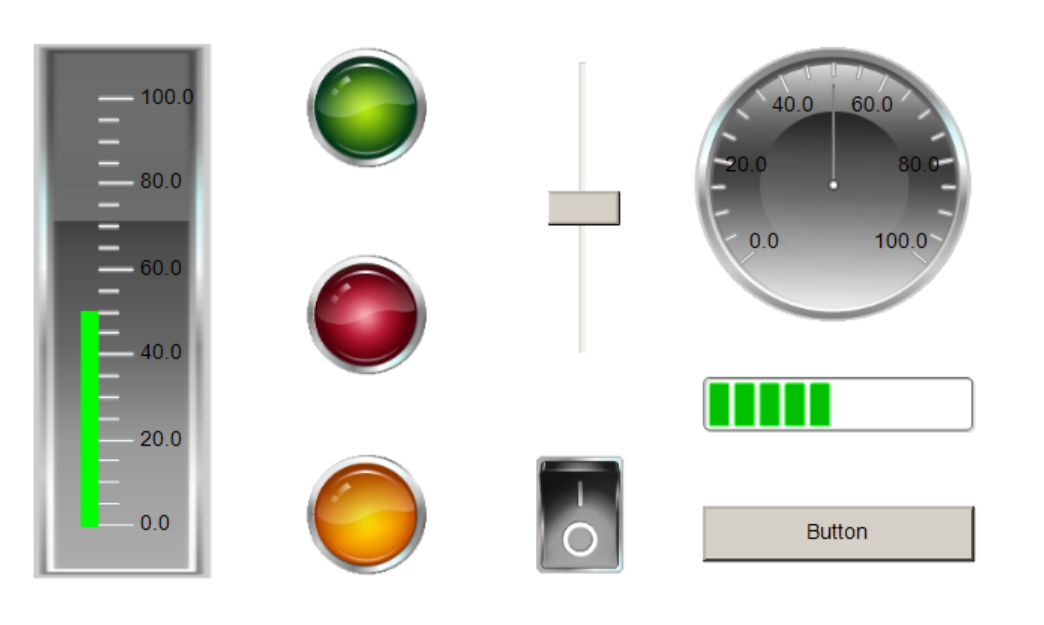
\includegraphics[width=0.8\textwidth]{Bilder/Codesys symbol.png}
    \caption{Eksempel Codesys visualisering}\label{fig:reaktorsoner}
\end{figure}

\newpage
